\documentclass{beamer}

\usepackage[latin1]{inputenc}
\usepackage{graphicx}
\usepackage{amssymb,amsmath}
%\usepackage{pslatex}
\usepackage{verbatim}
\usepackage{pst-all}
\usepackage{algorithmic}
\usepackage{multicol}

\usetheme{Goettingen}
\title[SDF]{Fault Tolerance for Cloud-Based Streaming Programs}
\author{Nic Hollingum \\ Supervisor: Dr. Bernhard Scholz}
\institute{USYD}
\begin{document}

\begin{frame}
\titlepage
\end{frame}

\begin{frame}{Outline}
\begin{itemize}
	\item Background
	\item Models and Systems
	\item Experiments
	\item Contributions and Future Work
\end{itemize}
\end{frame}

%-----------------------------------------------------------------------------------
\section{Background}

\begin{frame}{The Problem}
\begin{columns}
\begin{column}{6cm}
\begin{itemize}
	\item High performance computing
	\item Parallelisable paradigms
		\begin{itemize}
			\item Synchronous Dataflow (SDF)
		\end{itemize}
	\item Need for Fault Tolerance (FT)
	\item Opportunity for catering FT to SDF
\end{itemize}
\end{column}
\begin{column}{4cm}
	\center{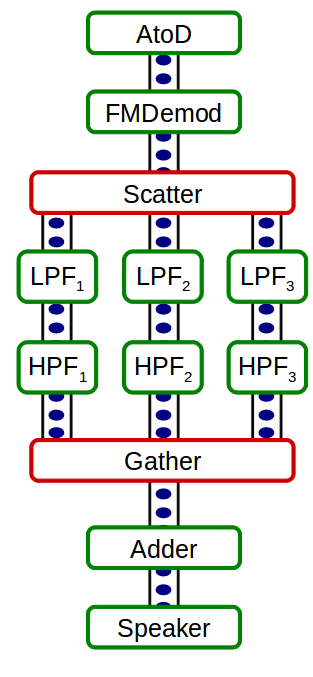
\includegraphics[width=4cm]{../res/multiradio.png}}
\end{column}
\end{columns}
\end{frame}

\begin{frame}{Related Work}
\begin{columns}
\begin{column}{5cm}
	\center{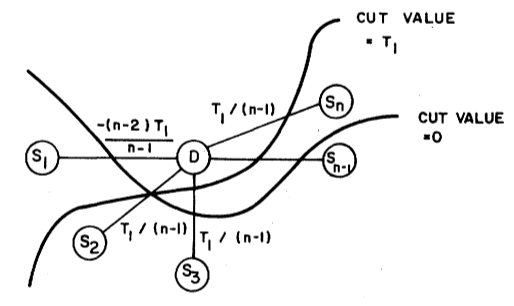
\includegraphics[width=5cm]{../res/multicut.png}}
\end{column}
\begin{column}{5cm}
\begin{itemize}
	\item Streaming Systems
		\begin{itemize}
			\item StreamIt \cite{thies10}
			\item S-Net \cite{pen09}
			\item InfoSphere, Spade \cite{ged08}
			\item DryadLINQ \cite{yu08}
		\end{itemize}
	\item Fault Tolerance
		\begin{itemize}
			\item Error Recovery (Databases) \cite{dbrec}
			\item Task Distribution \cite{lit07}
			\item Cloud-Recovery \cite{ree06}
		\end{itemize}
\end{itemize}
\end{column}
\end{columns}
\end{frame}

\begin{frame}{Research Goals}
\begin{itemize}
	\item How do we provide FT?
	\item What is the cost of ensuring FT?
	\item How do we implement the FT mechanisms?
	\item What guarantees can be made?
\end{itemize}
\end{frame}

%-----------------------------------------------------------------------------------
\section{Models and Systems}

\begin{frame}{AMPL Solver}
\begin{align}
	\nonumber \min & \sum_{a \in N; p \in P} \mathbf{I}_{a,p}\mathbf{X}_{a,p} + \sum_{a,b \in N; p,q \in P} \mathbf{C}_{a,b,p,q}\mathbf{Y}_{a,b,p,q} \\
	\nonumber s.t. &  \\
	\nonumber & \forall a \in N : \sum_{p \in P}\mathbf{X}_{a,p} = 1 \\
	\nonumber & \forall a,b \in N : \forall p,q \in P : \quad \mathbf{Y}_{a,b,p,q} \leq \mathbf{X}_{a,p} \\
	\nonumber & \forall a,b \in N : \forall p,q \in P : \quad \mathbf{Y}_{a,b,p,q} \leq \mathbf{X}_{b,q} \\
	\nonumber & \forall a,b \in N : \forall p,q \in P : \quad \mathbf{X}_{a,p} + \mathbf{X}_{b,q} - 1 \leq \mathbf{Y}_{a,b,p,q} \\
	\nonumber & \forall a,b \in N : \sum_{p \in P}\mathbf{Y}_{a,b,p,p}\mathbf{D}_{a,b} = 0
\end{align}
\end{frame}

\begin{frame}{Heuristic Solver}
\begin{columns}
\begin{column}{5cm}
\begin{itemize}
	\item NP-Hardness of problem
		\begin{itemize}
			\item Reduction from Multi-Terminal Cut problem
		\end{itemize}
	\item Greedy rounds-based algorithm
	\item Polynomial $O(n^2 p)$
		\begin{itemize}
			\item For each unit
			\item Choose the processor which has least total cost
			\item repeat
		\end{itemize}
\end{itemize}
\end{column}
\begin{column}{5cm}
	\center{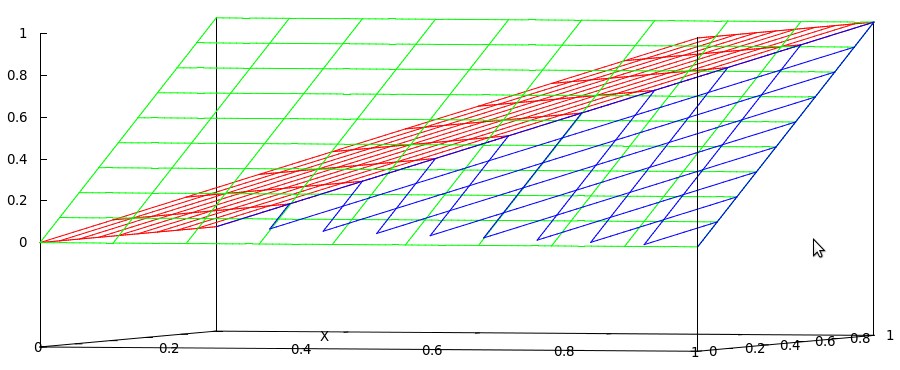
\includegraphics[width=5cm]{../res/approx.png}}
\end{column}
\end{columns}
\end{frame}

\begin{frame}{Simulator}
\begin{columns}
\begin{column}{5cm}
	\center{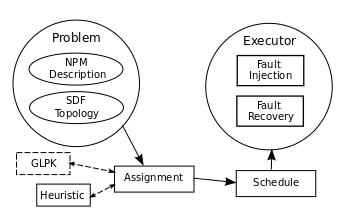
\includegraphics[width=5cm]{../res/sysDiagram.png}}
\end{column}
\begin{column}{5cm}
\begin{itemize}
	\item SDFSimulator, Java
	\item Threaded
	\item Arbitrary SDF graphs
	\item Actual execution
	\item Calls to heuristic and optimal solvers
\end{itemize}
\end{column}
\end{columns}
\end{frame}

%-----------------------------------------------------------------------------------
\section{Experiments}

\begin{frame}{Fault Tolerance}
\begin{itemize}
	\item Single Failure:
	\begin{itemize}
		\item Successful computations
		\item Replication shows no overhead
		\item Recomputation has restarting overhead
	\end{itemize}
	\item Multiple failure:
	\begin{itemize}
		\item Replication fails after enough processors go offline
		\item Recomputation excessively restarts
	\end{itemize}
\end{itemize}
\end{frame}

\begin{frame}{Optimality}
\begin{itemize}
	\item Small instances
	\item Heuristic assignment vs. Optimal assignment
	\item Heuristic performance stable over replications
	\item Heuristic performance degrades with larger problem sizes
	\item On average 10\% more than optimal
\end{itemize}
\end{frame}

%-----------------------------------------------------------------------------------
\section{Contributions and Future Work}

\begin{frame}{Contributions}
\begin{itemize}
	\item Formalised FT Mechanisms
	\item Developed AMPL Model
	\item Proved NP-Hardness
	\item Developed a Heuristic solver, shown to be 10\% worse
	\item Developed and experimented on SDFSimulator
\end{itemize}
\end{frame}

\begin{frame}{Future Work}
\begin{itemize}
	\item Parallelism
	\item Hybridising fault tolerance mechanisms
	\item Approximations
	\item Cloud deployment
\end{itemize}
\end{frame}

\begin{frame}[allowframebreaks]{References}
\bibliographystyle{plain}
\bibliography{biblio}
\end{frame}

\begin{frame}{Questions?}
\end{frame}

\end{document}
